\textbf{Taller con el Brazo Robótico SCORBOT-ER 4u}

Tomando como referencia el Brazo SCORBOT-ER 4u disponible en el laboratorio. Investigue sobre las características de este brazo e identifique los grados de libertad e intente identificar qué tipo de articulaciones encontramos en el Brazo SCORBOT-ER 4u. Utilizar recursos de apoyo como videos en la Web. 

\begin{figure}[H]
    \centering
    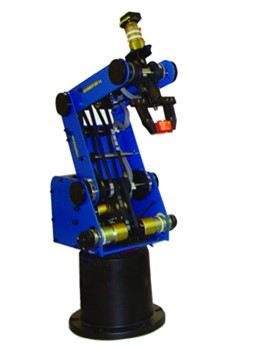
\includegraphics[scale = 0.5]{Imagenes/robot_p1.jpg}
    \caption{Figura1: Brazo SCORBOT-ER 4u }{Fuente: Profesor}
\end{figure}

El ScorBot ER-4U es un sistema versátil y confiable para la capacitación y educación en robótica industrial. El brazo robótico ScorBot ER-4U se puede montar sobre una mesa, un pedestal o una base deslizante lineal. La velocidad y repetibilidad del robot lo hacen muy adecuado tanto para operaciones independientes como para uso integrado en aplicaciones de celdas de trabajo automatizadas, como soldadura robótica, visión artificial, supervisión de máquinas CNC y otras operaciones FMS.

Su estructura mecánica es verticalmente aticulada. Este diseño permite que el efector final se posicione y oriente arbitrariamente dentro de un espacio de trabajo grande. Cuenta con 5 ejes de rotación (grados de libertad) y una pinza. Las características de sus ejes de rotación son:

\begin{table}[H]
    \centering
    \begin{tabular}{|c|c|c|}
        \hline
        Eje de Movimiento & Rango & Velocidad Efectiva \\
        \hline
        Rotación de la base & 310° & 20°/seg \\ 
        \hline
        Rotación del hombro & 158° & 26.3°/seg \\
        \hline
        Rotación del codo & 260° & 26.3°/seg \\
        \hline
        Inclinación de la muñeca & 260° & 83°/seg \\
        \hline
        Rotación de la muñeca & \parbox[c]{6cm}{Ilimitado (mecánicamente)\\±570° (eléctricamente)} & 106°/seg\\
        \hline
    \end{tabular}
    \caption{Características de los ejes del brazo}{Fuente: Internet}
\end{table}

\begin{figure}[H]
    \centering
    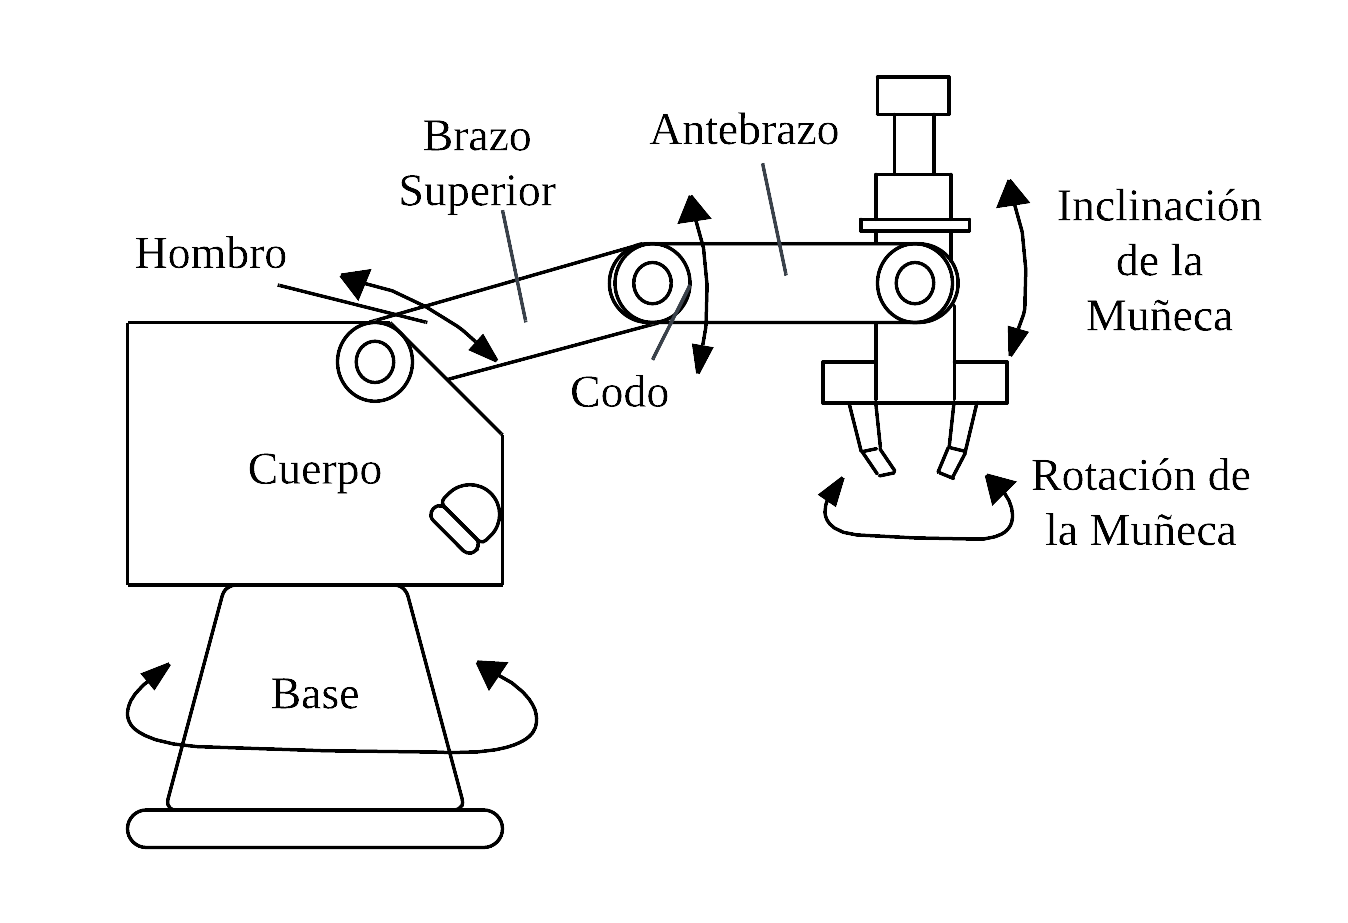
\includegraphics[scale = 0.5]{Imagenes/esquema_robot.png}
    \caption{Esquema del brazo SCORBOT-ER 4u}{Fuente: Propia}
\end{figure}